\chapter{Especificación del Diseño}

\section{Visión general}

	En este capítulo se describe el trabajo de diseño realizado para el proyecto, así como el entorno y las herramientas que han sido utilizadas para llevarlo a cabo.

\section{Arquitectura}

	La arquitectura básica del juego es la que se muestra en la siguiente imagen. El usuario genera entradas al juego mediante el teclado, después estas entradas son procesadas por la lógica del juego y se realizan las acciones pertinentes en función del estado del juego. Una vez actualizado el estado del juego ha sido actualizado, los módulos de audio y vídeo generan las salidas correspondientes y las muestran mediante la pantalla y el dispositivo reproductor de audio actual.

	\begin{figure}[!htp]
		 \centering
		 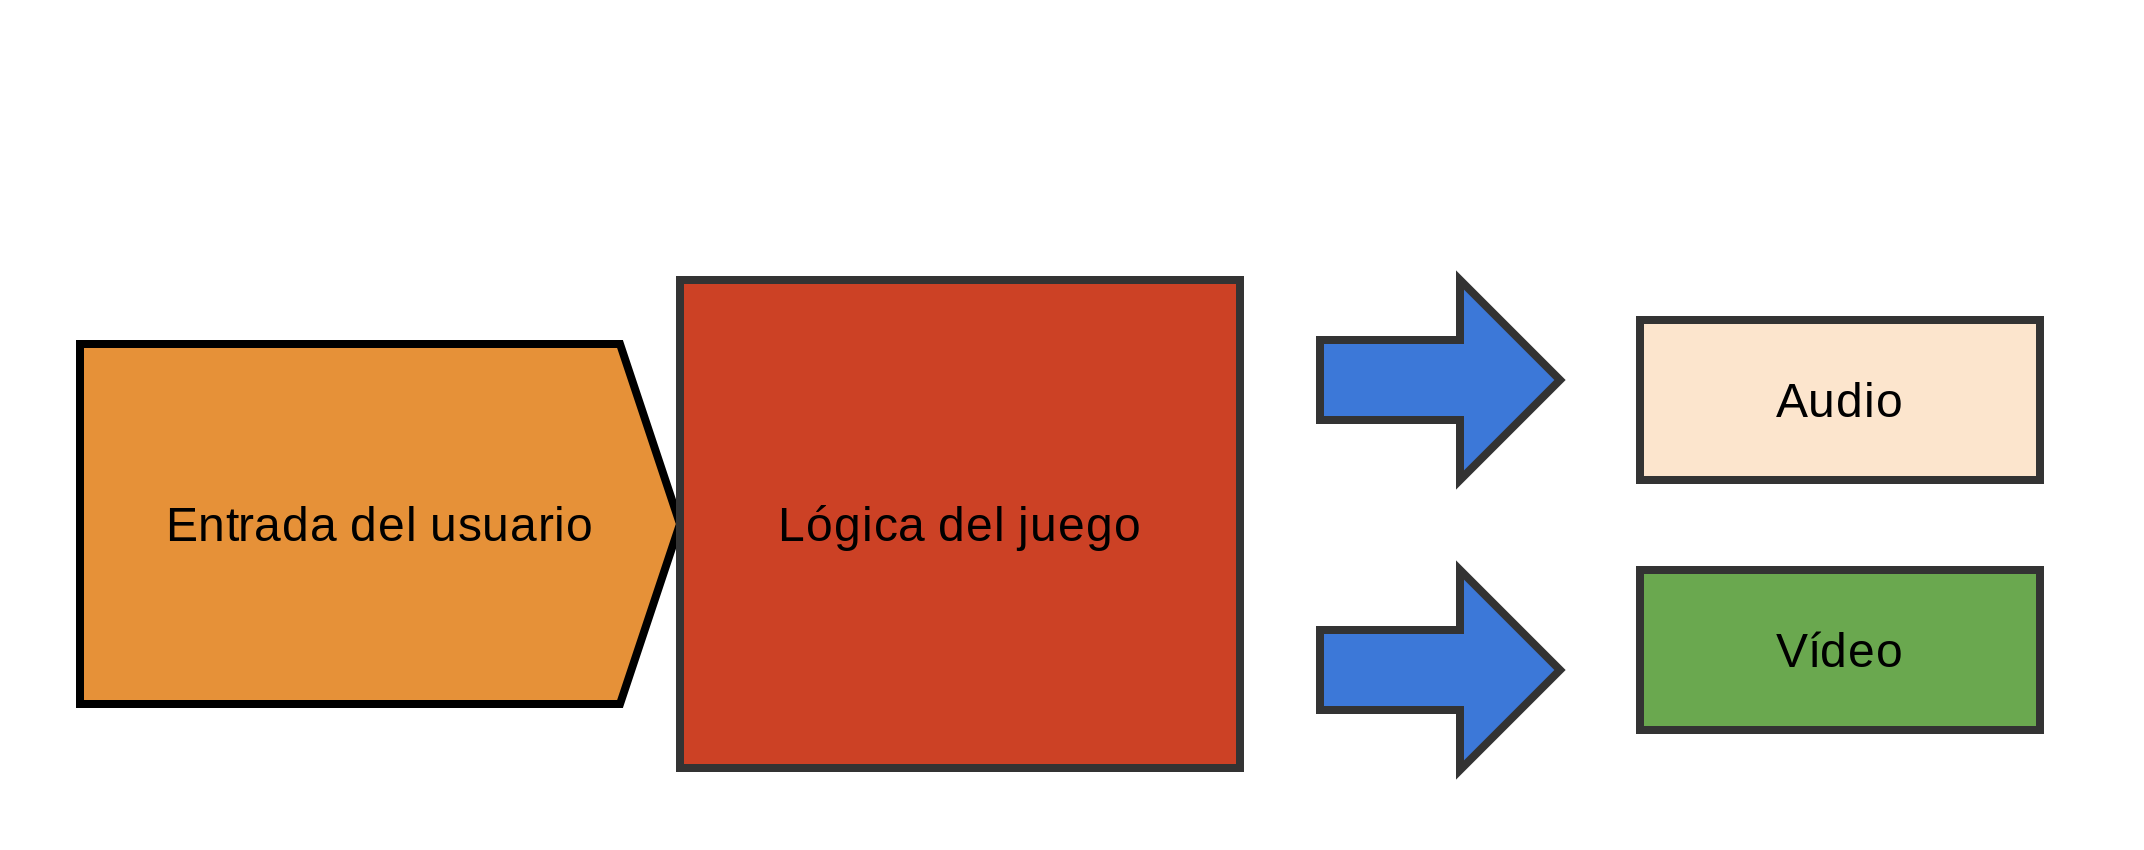
\includegraphics[scale=.15]{fig/architecture}
		 \caption{Diagrama de arquitectura}
		 \label{fig:arch}
	\end{figure}

	\FloatBarrier

\section{Diagrama de clases}

	\begin{figure}[!htp]
		 \centering
		 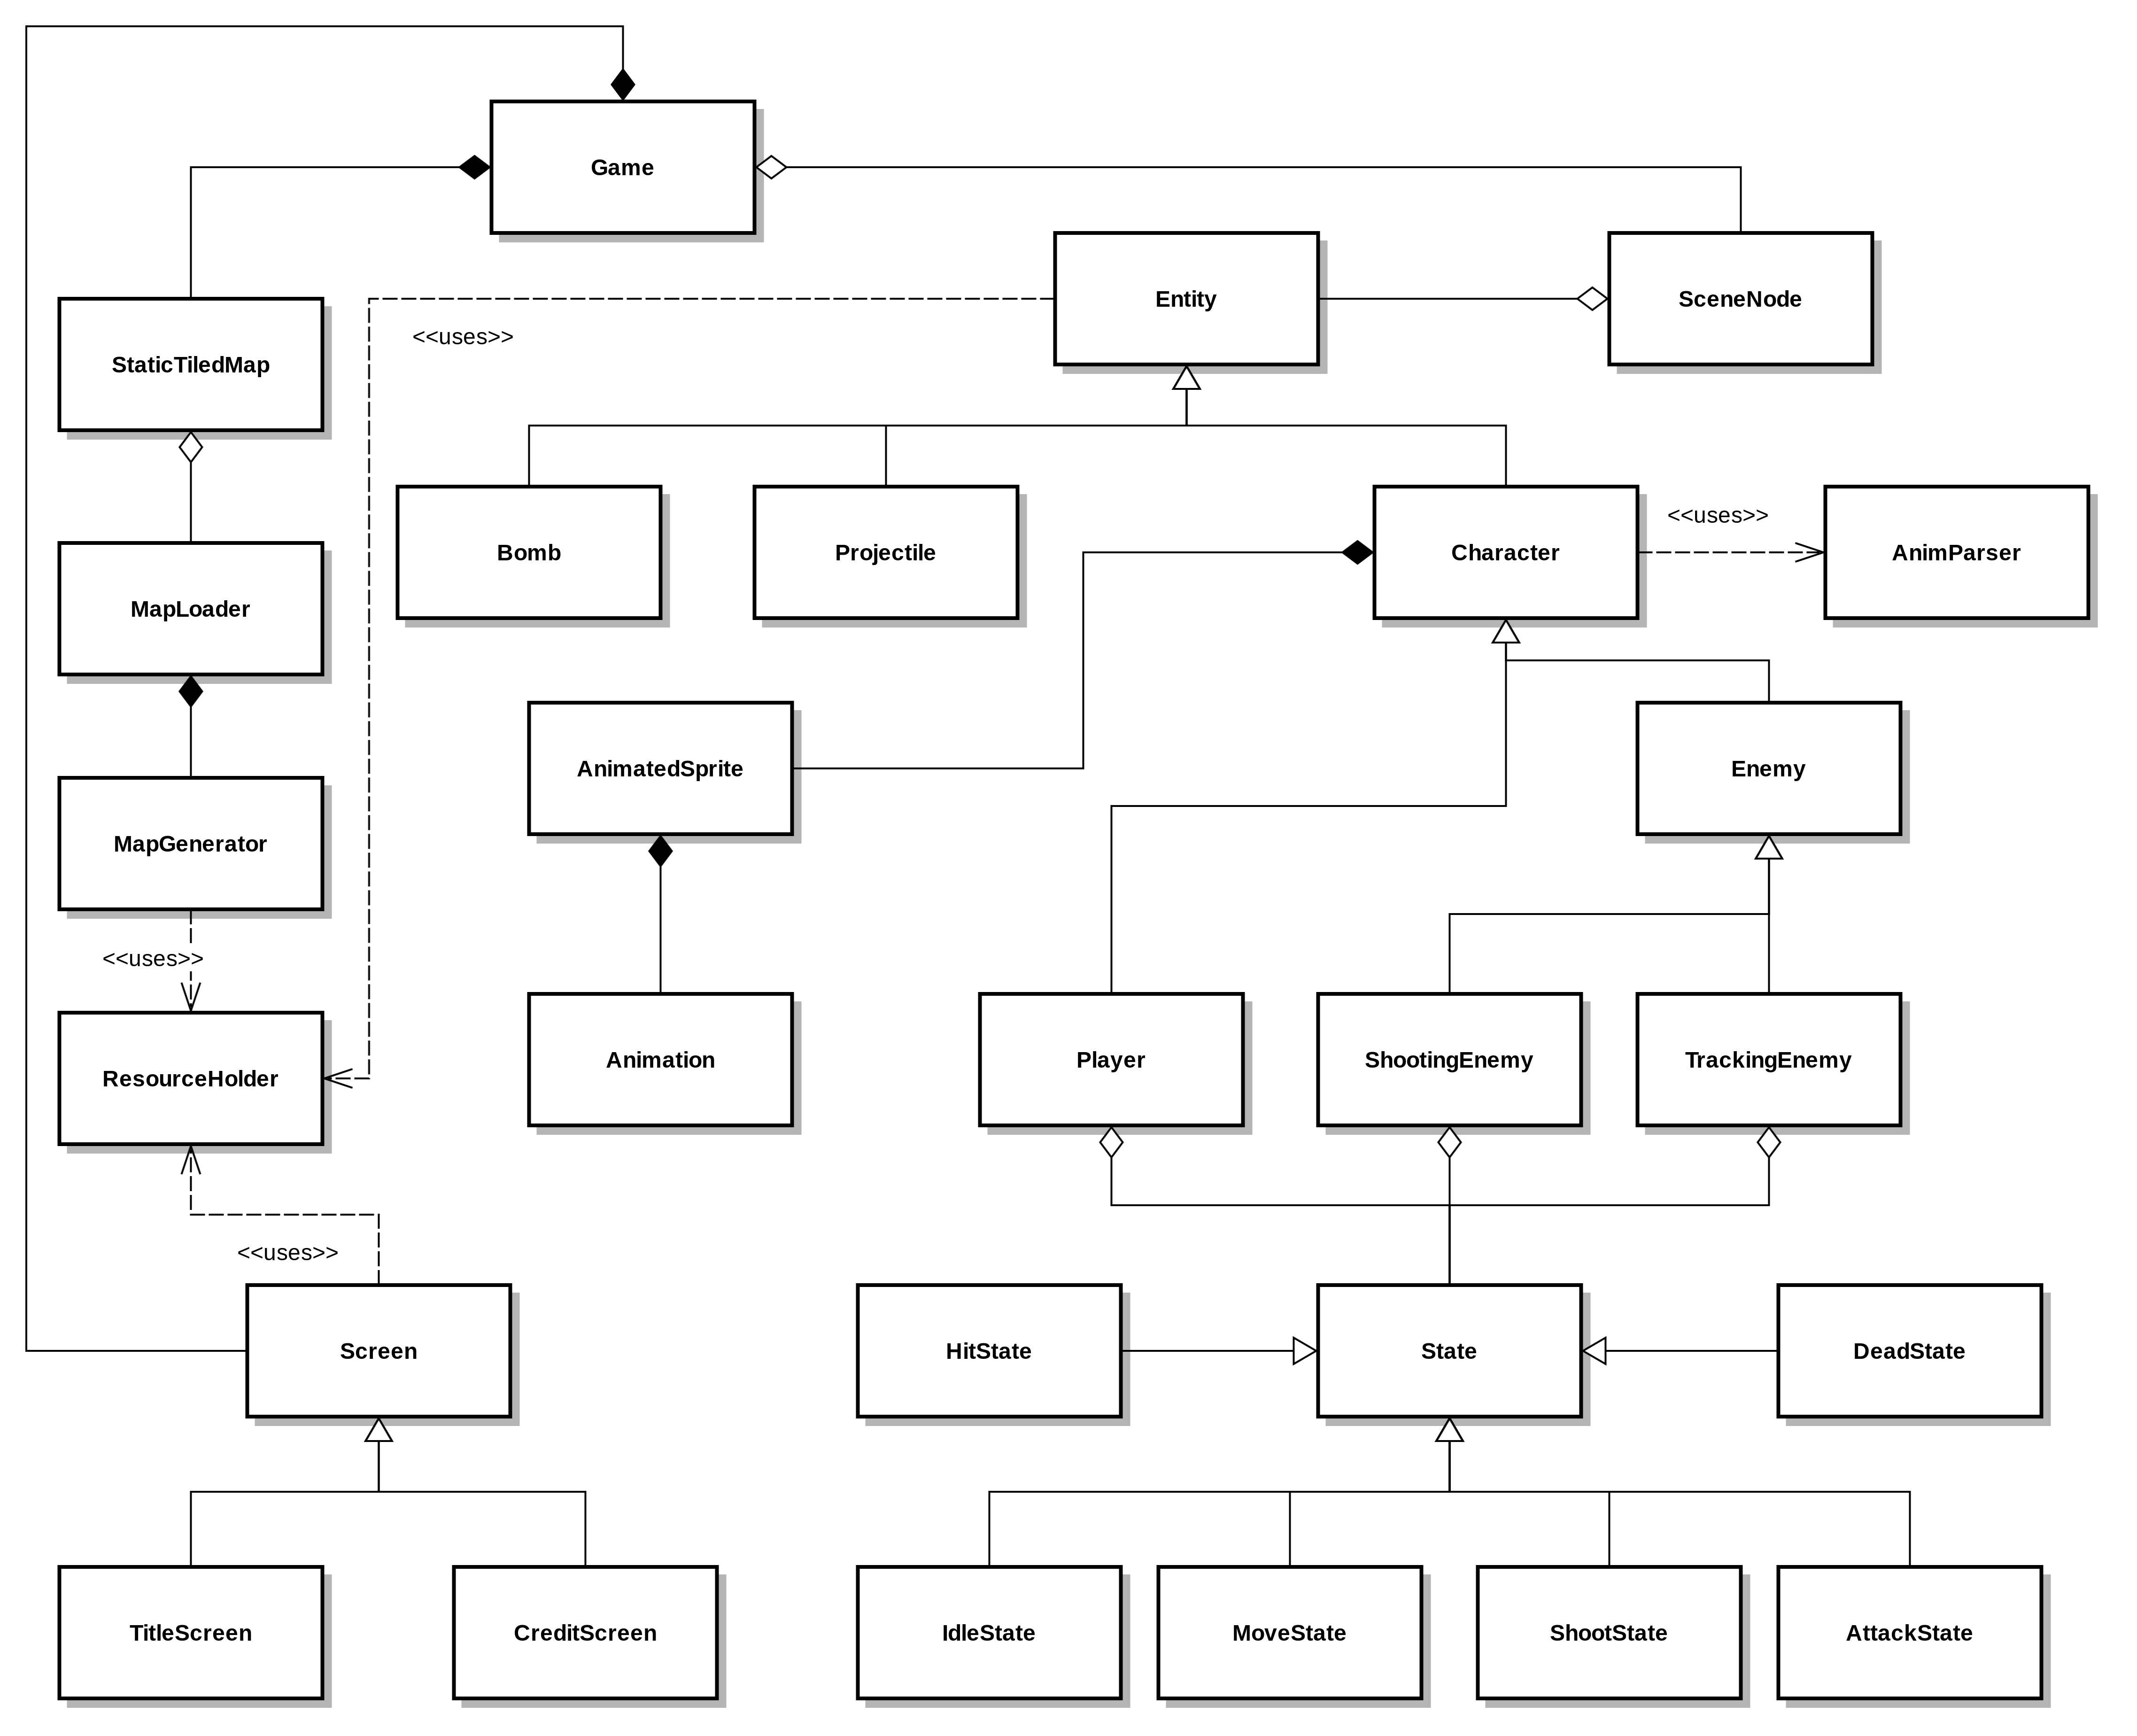
\includegraphics[scale=.05]{fig/class}
		 \caption{Diagrama de clases}
		 \label{fig:class}
	\end{figure}

	\FloatBarrier

\section{Diagramas de actividad}

	A continuación se muestra el diagrama de actividad del programa desde que se ejecuta hasta que finaliza.

	\begin{figure}[!htp]
		 \centering
		 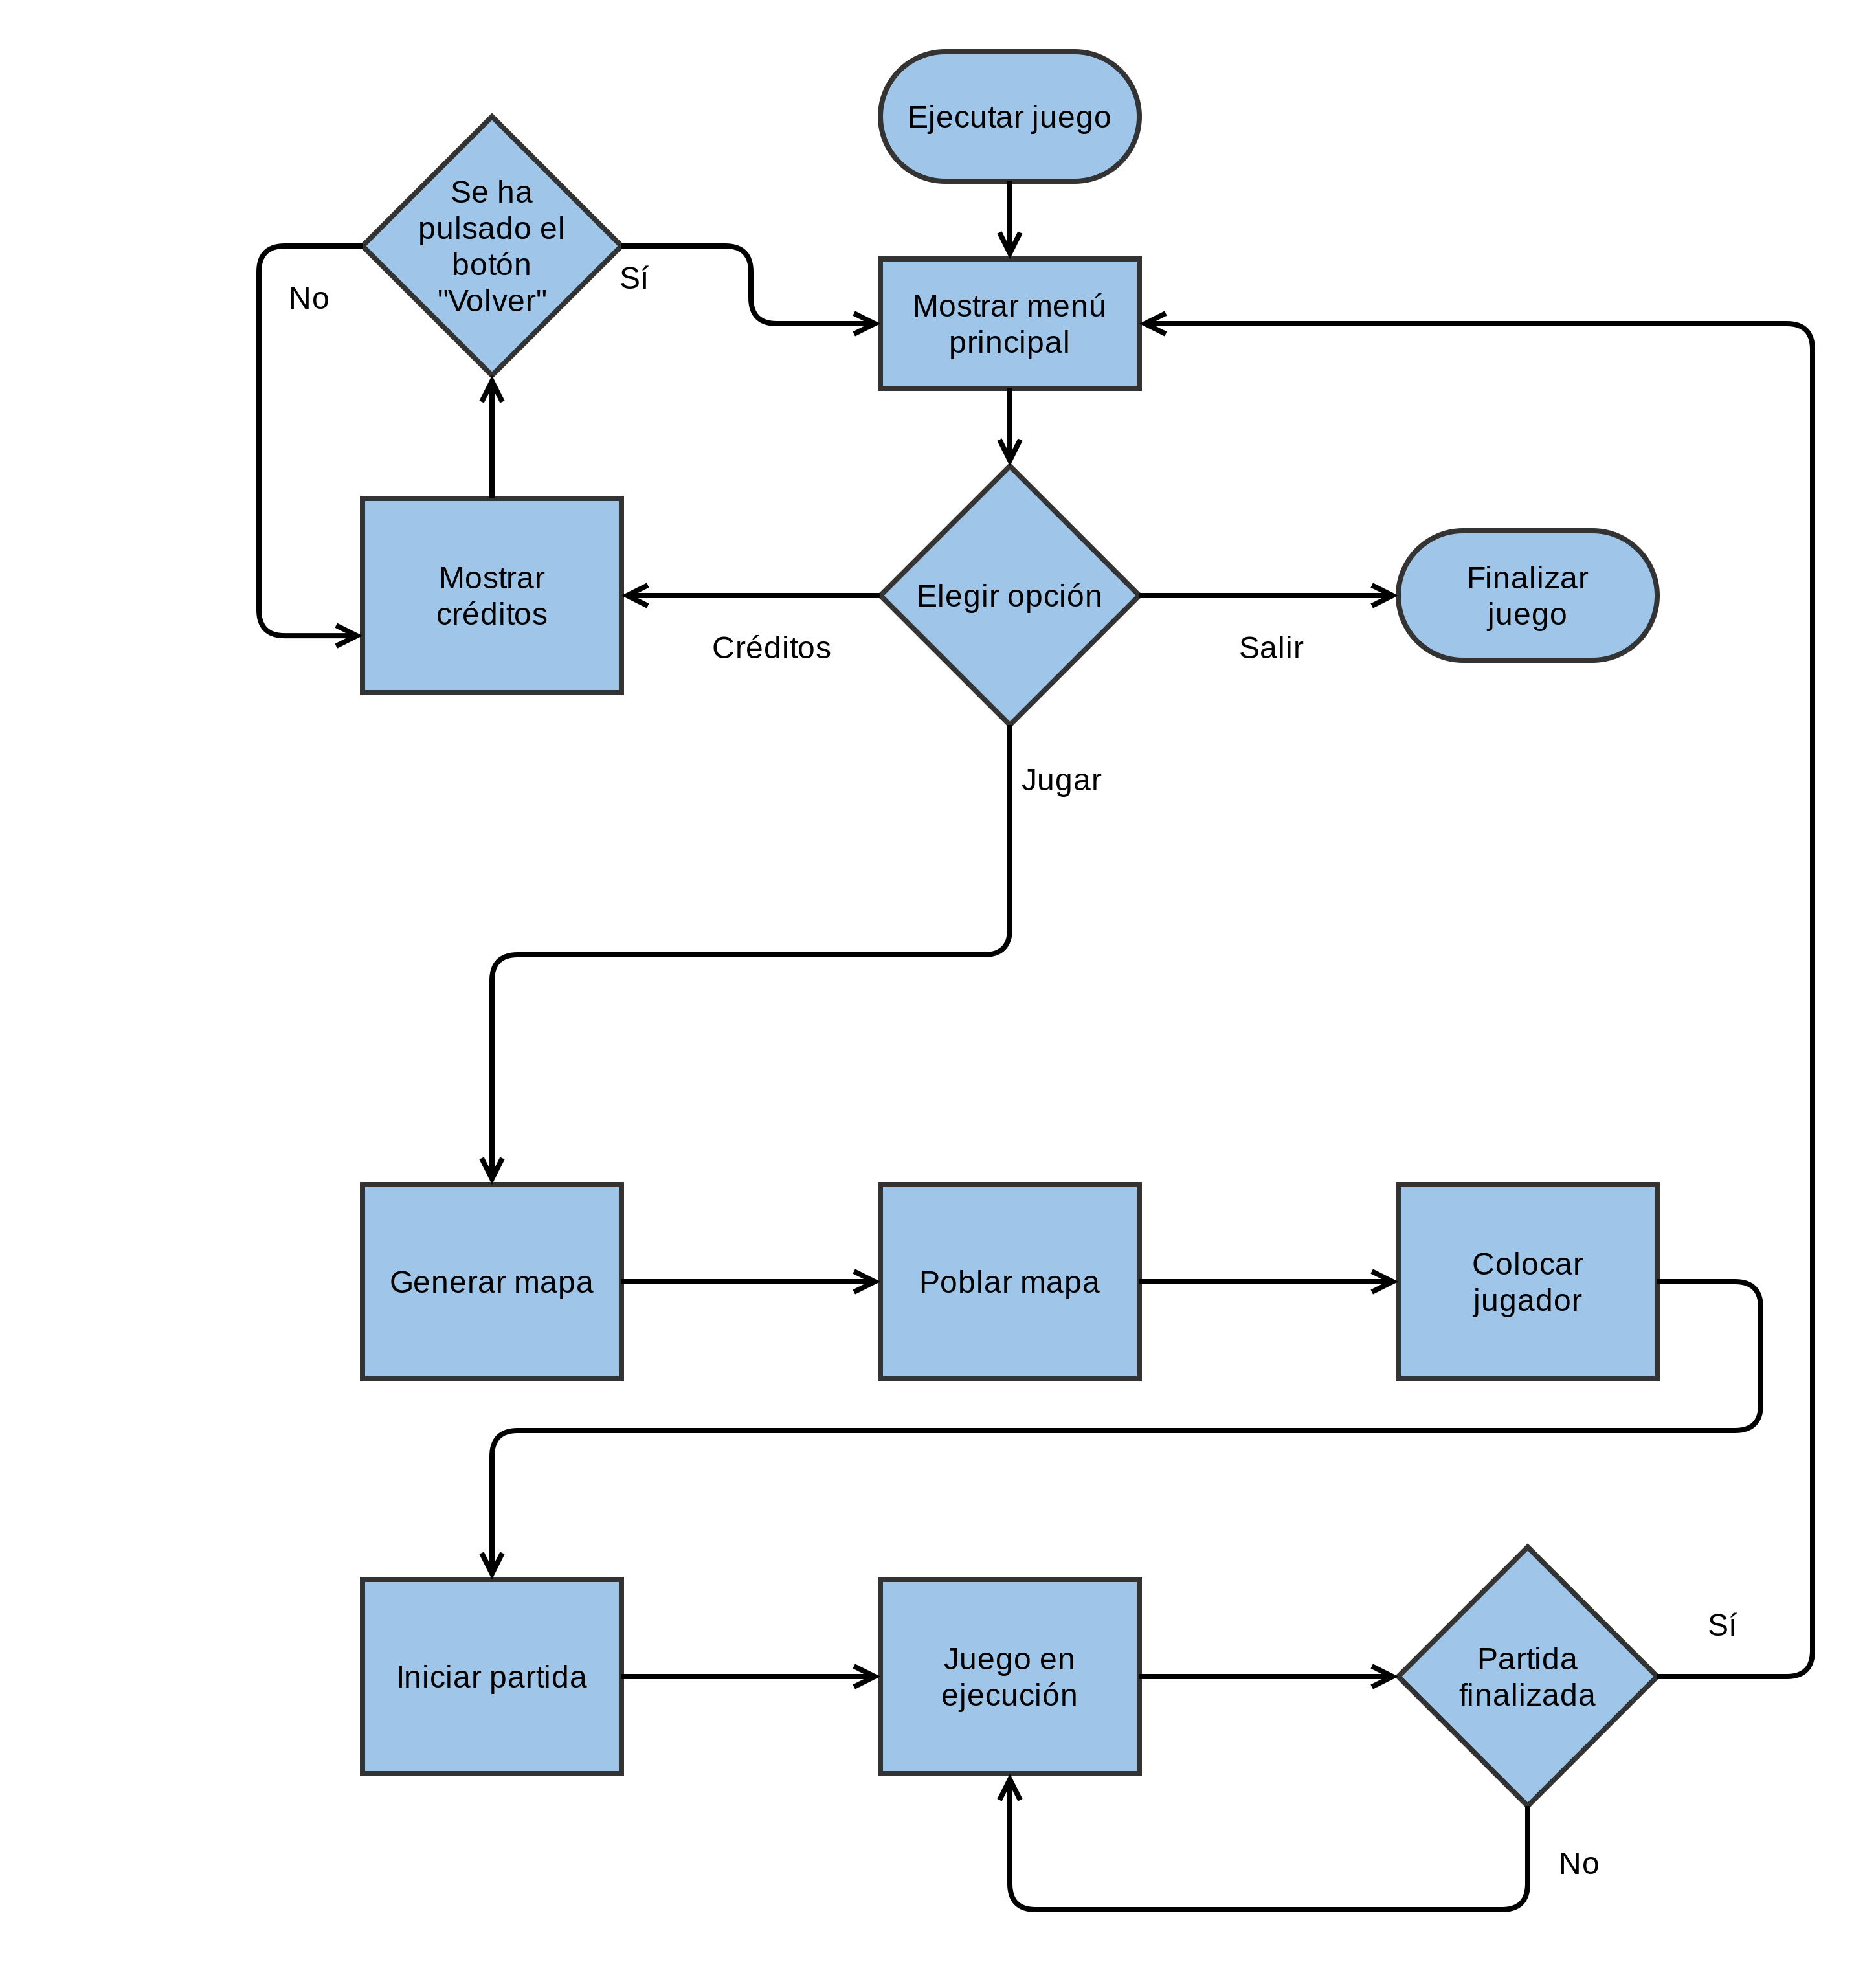
\includegraphics[scale=.15]{fig/actividad}
		 \caption{Diagrama de actividad}
		 \label{fig:activi}
	\end{figure}

	\FloatBarrier

\section{Tecnologías utilizadas}

	En este capítulo se describirán las tecnologías utilizadas para el desempeño del proyecto. Además, se dará una breve explicación de por qué han sido utilizadas y qué beneficios aportan al proyecto.

	\subsection{\acrshort{sfml}}

		\acrfull{sfml}~\cite{sfml} es una librería multiplataforma de desarrollo de software diseñada para proveer una interfaz simple a varios componentes multimedia en ordenadores. Está escrita en C++ con enlaces disponibles para C, D, Java, Python, Ruby, .NET, Go, Rust, OCaml, Euphoria y Nim. Existen también compilaciones experimentales para dispositivos móviles.

		\acrshort{sfml} gestiona tanto la creación e interacción de ventanas como de contextos \acrshort{opengl}. También provee de un módulo grñafico para gráficos acelerados por hardware en 2D el cual incluye representación de texto utilizando FreeType, un módulo de audio que se sirve de \acrshort{openal} y un módulo de conexión para comunicación básica por \acrshort{tcp} y \acrshort{udp}.

		\acrshort{sfml} es un software gratuito y de código libre provisto bajo los términos de la licencia zlib/png. Está disponible para Windows, Linux, OS X y FreeBSD.

		\begin{figure}[!htp]
			 \centering
			 
\includegraphics[scale=.8]{fig/sfml}
			 \caption{Logotipo de \acrshort{sfml}}
			 \label{fig:sfml}
		\end{figure}

		\FloatBarrier

		Se ha decidido utilizar \acrshort{sfml} en el proyecto ya que uno de los objetivos del mismo es aprender a crear una arquitectura software apropiada para videojuegos, de forma que los motores con editor visual no eran una opción, al abstraer al usuario de ella. A pesar de que la librería de referencia para este tipo de aplicaciones es \acrshort{sdl}, se ha decidido usar \acrshort{sfml} ya que a diferencia de la primera, la cual está escrita en C, \acrshort{sfml} está escrita en C++ y concebida con orientación a objetos. Esto supone una ventaja ya que el proyecto ha sido desarrollado en C++ y el paradigma de programación utilizado ha sido el de la orientación a objetos.

	\subsection{C++}

		C++~\cite{cpp} es un lenguaje de programación de propósito general. Tiene características de programación imperativa, orientada a objetos y genérica, mientras provee facilidades para la manipulación de memoria a bajo nivel.

		Está diseñado pensando en la programación de sistemas, sistemas embebidos, sistemas con recursos limitados y grandes sistemas, con el rendimiento, la eficiencia y la flexibilidad de uso como sus requisitos de diseño. C++ también ha sido útil en otros muchos contextos, siendo fortalezas clave la infraestructura de software y aplicaciones con recursos limitados, incluyendo aplicaciones de escritorio, servidores, aplicaciones de rendimiento crítico y software de entretenimiento. C++ es un lenguaje compilado, con implementaciones del mismo disponibles en muchas plataformas y provistas por varias organizaciones, incluyendo \acrshort{fsf}, \acrshort{llvm}, Microsoft e Intel.

		C++ está estandarizado por \acrshort{iso}, con la última versión estándar ratificada y publicada por \acrshort{sfml} en diciembre de 2014 como \acrshort{iso}/\acrshort{iec} 14882:2014 (informalmente conocida como C++14). Muchos otros lenguajes de programación han sido influenciados por C++, entre los que se encuentran C\#, Java, y versiones posteriores a 1998 de C.

		\begin{figure}[!htp]
			 \centering
			 
\includegraphics[scale=.25]{fig/cpp}
			 \caption{Logotipo de C++}
			 \label{fig:cpp}
		\end{figure}

		\FloatBarrier

		Se ha decidido utilizar C++ para el desarrollo del proyecto ya que es el lenguaje estándar de la industria, y dado que el producto busca competir, es importante que esté hecho con las mejores herramientas. C++ es en este caso dicha herramienta, por su eficiencia y flexibilidad.

	\subsection{\acrshort{json}}

		\acrfull{json}~\cite{json} es un formato estándar abierto que usa texto legible por humanos para transmitir objetos de información consistentes en pares atributo-valor. Es principalmente utilizado para transmitir información entre un servidor y una aplicación web como alternativa a \acrshort{xml}.

		Aunque originalmente fue derivado del lenguaje de programación Javascript, \acrshort{json} es un formato de datos independiente del lenguaje. El código necesario para generar y analizar información en \acrshort{json} está disponible en muchos lenguajes de programación.

		\begin{figure}[!htp]
			 \centering
			 
\includegraphics[scale=.5]{fig/json}
			 \caption{Logotipo de \acrshort{json}}
			 \label{fig:json}
		\end{figure}

		\FloatBarrier

		Se ha decidido utilizar \acrshort{json} frente a \acrshort{xml} porque el equipo disponía de experiencia previa con \acrshort{json} y no con \acrshort{xml}. Ambas tecnologías ofrecen características similares, pero \acrshort{json} es más simple y por tanto más fácil de mantener.

	\subsection{\acrshort{tgui}}

		\acrfull{tgui}~\cite{tgui} es una librería de GUI multiplataforma en C++ para \acrshort{sfml}. Entre sus características más destacables encontramos la facilidad de uso, la portabilidad de código, la posibilidad de modificar interfaces sin necesidad de recompilar, un gestor de texturas externo que evita la recarga de imágenes y está provisto bajo la misma licencia que \acrshort{sfml}, zlib/png.

		\begin{figure}[!htp]
			 \centering
			 
\includegraphics[scale=.75]{fig/tgui}
			 \caption{Logotipo de \acrshort{tgui}}
			 \label{fig:tgui}
		\end{figure}

		\FloatBarrier

		Se ha decidido utilizar \acrshort{tgui} en el proyecto para agilizar el desarrollo de las interfaces de usuario. Hubiese sido posible crear una implementación propia con los elementos necesarios, pero hubiese consumido recursos que eran de gran valor para otros apartados del proyecto.

	\subsection{JsonCpp}

		JsonCpp~\cite{jsoncpp} es una librería C++ que permite manipular documentos \acrshort{json}, incluyendo serialización y deserialización a y desde cadenas de texto. También preserva comentarios existentes en los pasos de serialización y deserialización, haciendo el formato conveniente para archivos generados por usuarios.

		De entre las distintas opciones para trabajar con \acrshort{json} en C++, se ha decantado por esta ya que su integración en el proyecto era muy sencilla, al igual que su uso.

\section{Diseño del juego}

	En esta sección se presentará el diseño del juego, es decir, la definición del comportamiento del mismo dentro de una partida.

	\subsection{Jugador}

		El jugador podrá moverse libremente por el mapa y utilizar cualquiera de sus habilidades en todo momento, siempre que no esté ya usando una o esté siendo desplazado por haber sido alcanzado por un ataque enemigo. No existirá límite en el número de veces que puede usar cualquiera de sus habilidades.

		Si el jugador es dañado, su barra de vida, la cual siempre será visible durante una partida, se reducirá en un cuarto. De esta manera, si el jugador es dañado cuatro veces en la misma partida, morirá y la partida se considerará un fracaso. No existirá manera de regenerar la barra de vida.

		El enemigos dispone de tres habilidades: ataque cuerpo a cuerpo, disparo y poantar bomba. Si un jugador colisiona con un enemigo mientras ejecuta el ataque cuerpo a cuerpo y el lado de la colisión coincide con el lado hacia el que está ejecutando el ataque, el enemigo será dañado y el jugador quedará impune. En cualquier otro caso si el jugador es alcanzado por un enemigo o un proyectil enemigo, será dañado.

	\subsection{Enemigos}

		Habrá dos tipos de enemigo en el juego, ambos con el objetivo de acabar con el jugador. Ambos estarán quietos hasta que el jugador entre en su radio de acción, y se quedarán quietos si el jugador sale del mismo.

		El primer enemigo buscará chocarse contra el jugador, de forma que buscará la ruta más corta hasta el mismo y procederá a recorrerla. En caso de que el jugador se mueva volverá a buscar una ruta hasta él. Si el enemigo colisiona con el jugador, lo dañará y lo empujará hacia atrás. Este enemigo morirá si es alcanzado por cualquiera de las habilidades del jugador.

		El segundo enemigo, en vez de buscar una ruta hasta el jugador, buscará la ruta más corta para alienarse con él y la recorrerá. Una vez alineado, disparará al jugador infinitas veces, con un breve espacio de tiempo entre disparo y disparo. Los disparos de este enemigo no podrán ser bloqueados o eliminados de ninguna manera, solo podrán ser esquivados. Este enemigo morirá si es alcanzado por cualquiera de las habilidades del jugador, y tanto sus disparos como su contacto físico directo dañarán al jugador y lo empujarán.

	\subsection{Colisiones con el mundo}

		Tanto el personaje como los enemigos deben colisionar adecuadamente con el mundo, es decir, solo deben ser capaces de atravesar las celdas que, tanto a nivel lógico como visual, son navegables. En caso de que intenten atravesar una celda que no cumpla alguno de los requisitos, el juego debe parar su movimiento y colocarlo justo al lado de la casilla que pretendía atravesar.

	\subsection{Colisiones con objetos}

		Habrá dos objetos con los que se pueda colisionar: proyectiles y bombas.

		Los proyectiles no colisionarán con el mundo, es decir, serán capaces de atravesar cualquier obstáculo. Los proyectiles lanzados por el jugador solo dañarán a enemigos y viceversa.

		Las bombas no podrán ser colocadas en partes del mapa que no se puedan atravesar. Una vez colocadas, permanecerán inactivas un breve periodo de tiempo, y tras esto explotarán. Mientras la bomba está inactiva, no tendrá ninguna consecuencia colisionar con ella. No obstaculizará el movimiento y no dañará. Sin embargo, a la hora de explotar, la caja de colisión de la bomba aumentará y dañará a cualquier cosa que colisione con ella, ya sea un enemigo o el propio jugador.

	\subsection{Objetivo}

		El objetivo del juego es eliminar a todos los enemigos del mapa dentro del tiempo límite fijado. Este tiempo será visible en todo momento en pantalla, y su valor se actualizará cada segundo. Se considerará una partida existosa si el jugador consigue acabar con todos ellos, y se considerará un fracaso si los enemigos consiguen matarlo o se le agota el tiempo límite.

\section{Plan de Pruebas}

	Durante la realización del proyecto han habido muchas pruebas para garantizar la calidad del código e intentar minimizar al máximo los errores. En este capítulo se explican las pruebas hechas.

	En la siguiente lista se muestran los tipos de prueba que se han hecho:

	\begin{itemize}
		\item \textbf{Pruebas unitarias:}
			
		Descripción de las pruebas unitarias llevadas a cabo en el proyecto.

		\item \textbf{Pruebas de integración:}
			
		Descripción de las pruebas de integración llevadas a cabo.

		\item \textbf{Pruebas de hardware:}
			
		Descripción de las pruebas de hardware realizadas.

		\item \textbf{Pruebas de usabilidad:}
			
		Descripción de las pruebas de usabilidad realizadas.
	\end{itemize}

	\subsection{Pruebas unitarias}

		A lo largo del proyecto se han realizado muchas pruebas unitarias. Estas consisten en dividir el código a partes mínimas para garantizar que el funcionamiento del mismo es el esperado. La realización de estas pruebas han sido enfocadas a la búsqueda de errores en los siguientes elementos:

		\begin{itemize}
			\item \textbf{Condiciones booleanas:} verificar el comportamiento del sistema al finalizar y asegurar que las variables evaluadas tienen asignados los valores esperados.

			\item \textbf{Indices de matrices:} verificar que en ningún momento se accede a posiciones fuera del rango de las matrices.

			\item \textbf{Comprobar valores nulos:} comprobar que donde se espera que haya una instancia de una clase verdaderamente la haya, de forma que el valor no sea nulo.

			\item \textbf{Operaciones de conversión:} asegurar que la conversión de un tipo a otro de datos es la apropiada, reforzando el código para que una conversión inadecuada cause un error en la aplicación.

			\item \textbf{Condiciones alternativas:} garantizar que al menos una rama es siempre satisfecha.

			\item \textbf{Iteraciones:} asegurar que las condiciones sean correctas de forma que nunca se generen bucle infinitos.

			\item \textbf{Impresión de secuencia:} utilizada para comprobar si la aplicación ejecuta bucles o condicionales imprimiendo la secuencia en consola.
		\end{itemize}

	\subsection{Pruebas de integración}

		La realización de estas pruebas consiste en garantizar que el funcionamiento de cada módulo sea correcto. Los módulos han sido probados de distintas maneras para asegurar que siempre se ejecutaban satisfactoriamente. Además, se han hecho pruebas que verifican que las interfaces de comunicación entre distintos módulos son correctas. Se ha prestado especial atención a este apartado para evitar que el error de un módulo pudiera propagarse a toda la aplicación, evitando así fallos en cadena.

	\subsection{Pruebas de hardware}

		Cuando el producto se encontraba en sus etapas finales, se ha procedido a compilar y ejecutar el juego en distintas configuraciones de hardware para comprobar que funcionaba correctamente. Gracias a la colaboración de compañeros y amigos ha habido posibilidad de probar el producto en una gama variada de hardware. En total se ha compilado y ejecutado el juego satisfactoriamente en catorce configuraciones distintas. Además, estas configuraciones disponían de distintos sistemas operativos, entre los que se encuentran Ubuntu, Linux Mint, Windows 7, Windows 8.1 y OS X. Esto demuestra que el código generado por el proyecto es multiplataforma.

	\subsection{Pruebas de usabilidad}

		Una parte fundamental de los juegos es la experiencia de usuario. Para conseguir la mejor posible, se ha contado con la colaboración de distintas personas que han ayudado a calibrar distintos menúes e interfaces gráficas. Las pruebas consistían en sesiones cortas de juego, en las que los usuarios compartía sus observaciones respecto a la interfaz y usabilidad general. Gracias a las opiniones recogidas, se han ajustado las posiciones y los tamaños de los elementos de la interfaz gráfica para acomodarlos a la mayoría de los usuarios. Por otro lado, se han ajustado los menús para ser más intuitivos.
